% Graph figures for the embodied-sensor paper. One figure environment per graph
% figure written by papers/embodied_sensor/make_graph_figures.py (g1 to g6) and
% the roles-by-edges readout fig6 from papers/embodied_sensor/make_figures.py.
%
% Every number in every caption is drawn on the figure from an artefact under
% divergence_study_outputs/ and verified by `make_graph_figures.py --check`
% (674 plotted values, 25 cross-artefact equalities, 1 record quote checked
% against the prereg text, run 2026-09-13). The comment after each caption
% names the artefact keys and the prereg RESULTS lines (L n in
% Guidance_Documents/prereg_embodiment_community.md) that carry each number.
%
% Citation keys. Every key cited below is in references.bib. The sixteen
% game-theory entries (milgrom1986relying, lipman1995robust,
% shin1998adversarial, dewatripont1999advocates, battaglini2002multiple,
% gentzkow2017competition, feddersen1998convicting, chwe1994farsighted,
% krishna2001model, myerson1986multistage, okunofujiwara1990strategic,
% glazer2004optimal and four more) were fetched at primary URLs on 2026-09-12,
% re-fetched on 2026-09-13, and merged into references.bib on 2026-09-13 from
% advocacy_refs.bib, which is kept as the fetch log.
%
% House style. No em dashes, no colons or semicolons in running prose, no lists.

\begin{figure}[t]
\centering
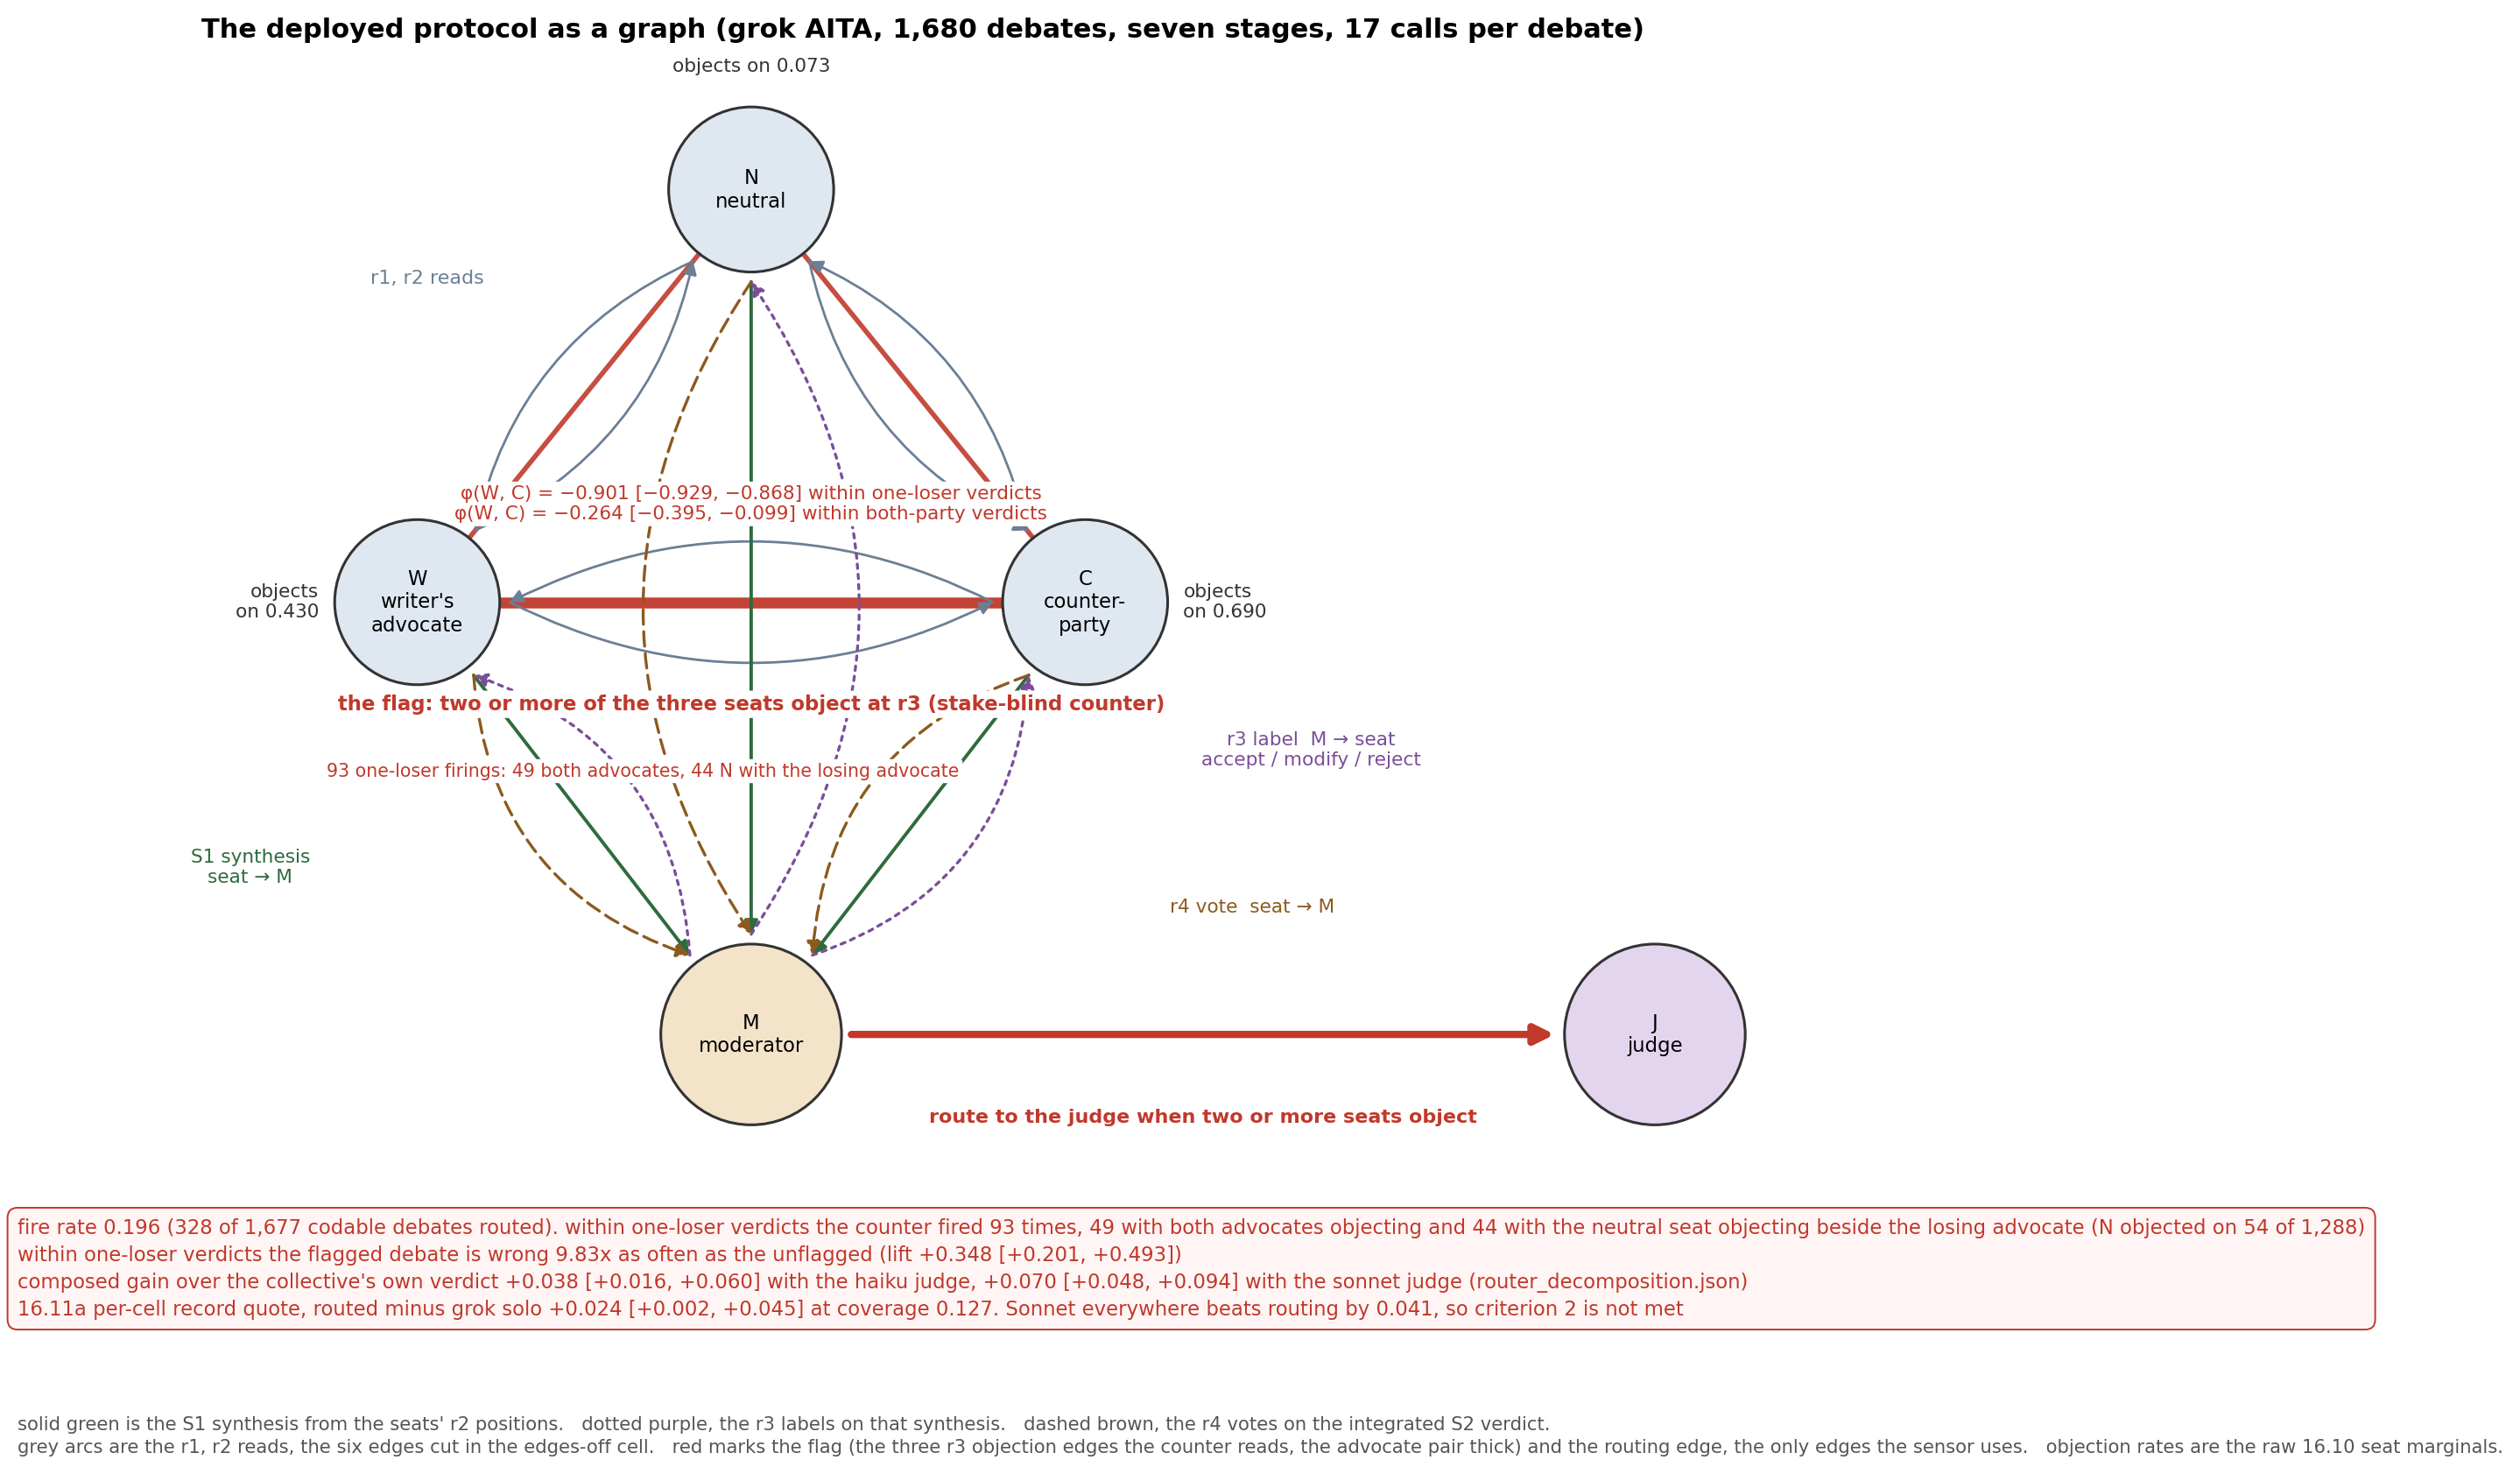
\includegraphics[width=\linewidth]{figures/g1_protocol.png}
\caption{The deployed protocol as a graph on grok AITA, 1,680 debates, seven
stages and 17 calls per debate. Five nodes, the writer's advocate W, the
counterparty C, the neutral adjudicator N, the moderator M and the routing
judge J. Grey arcs are the six r1 and r2 reads among the seats, the edges cut
in the edges-off cell. Green, purple and brown edges are the S1 synthesis, the
r3 labels and the r4 votes, the star every cell keeps. Red marks the only
edges the sensor uses. The flag is the three-seat set of r3 objections the
stake-blind counter reads, drawn as the three objection edges W to C, W to N
and C to N, and the counter fires when two or more of the three seats object.
The advocate pair is drawn thick because its against-interest crossings carry
the signal, but it is not the whole flag. Within one-loser verdicts the
counter fired on 93 debates, on 49 of them both advocates objected, and on the
other 44 the neutral seat objected beside the losing advocate (N objected on 54
of 1,288). The routing edge from M to J fires when the counter does. The
advocate edge is anti-correlated at $\phi$ $-0.901$ $[-0.929, -0.868]$ within
one-loser verdicts and collapses to $-0.264$ $[-0.395, -0.099]$ within
both-party verdicts. The counter fires on 0.196 of debates, and within
one-loser verdicts a flagged debate is wrong 9.83 times as often as an
unflagged one, lift $+0.348$ $[+0.201, +0.493]$. Routing the flagged debates to a judge adds
$+0.038$ $[+0.016, +0.060]$ over the collective's own verdict with the haiku
judge and $+0.070$ $[+0.048, +0.094]$ with the sonnet judge. Routing grok
alone to sonnet on the same flag beats grok alone by $+0.024$
$[+0.002, +0.045]$ at coverage 0.127 and loses to sonnet everywhere by 0.041,
so the judge edge is a cost-efficient cascade and not an accuracy ceiling.}
% make_graph_figures.py g1, emergent_graphs.json protocol.nodes / stages / edges
% (17 edges, six reads, the flag at protocol.edges[15] as a three-seat
% hyperedge with seats W, C, N since 2026-09-13) and communities.grok_aita.
% the 93 / 49 / 44 / 54 split from protocol.annotations.one_loser_firings_split,
% cross-checked under --check against graphs.one_loser (fire_rate.n_fired,
% edges."advocate_1|advocate_2".table.both, nodes.third.n_objected).
% phi one-loser and both-party from
% populations.s2_codable.graphs.{one_loser, both_party}.edges."advocate_1|advocate_2".phi
% (prereg L5003, L3666 to L3668). fire rate 0.196 L4149 (protocol.annotations.fire_rate_raw
% == communities.grok_aita.raw.fire_rate). 9.83x and lift +0.348 L4275
% (router_decomposition.json counter_lift_by_stratum.one_loser). composed gains
% L4299 and L4322 (router_decomposition.json composed_haiku / composed_sonnet
% paired_deltas.counter_minus_collective_alone). 16.11a per-cell routing gain
% L3621 and L3623, carried in protocol.annotations.routing_gain_over_solo_16_11a
% as a flagged record quote because no script reproduces it.
\label{fig-g1-protocol}
\end{figure}

\begin{figure}[t]
\centering
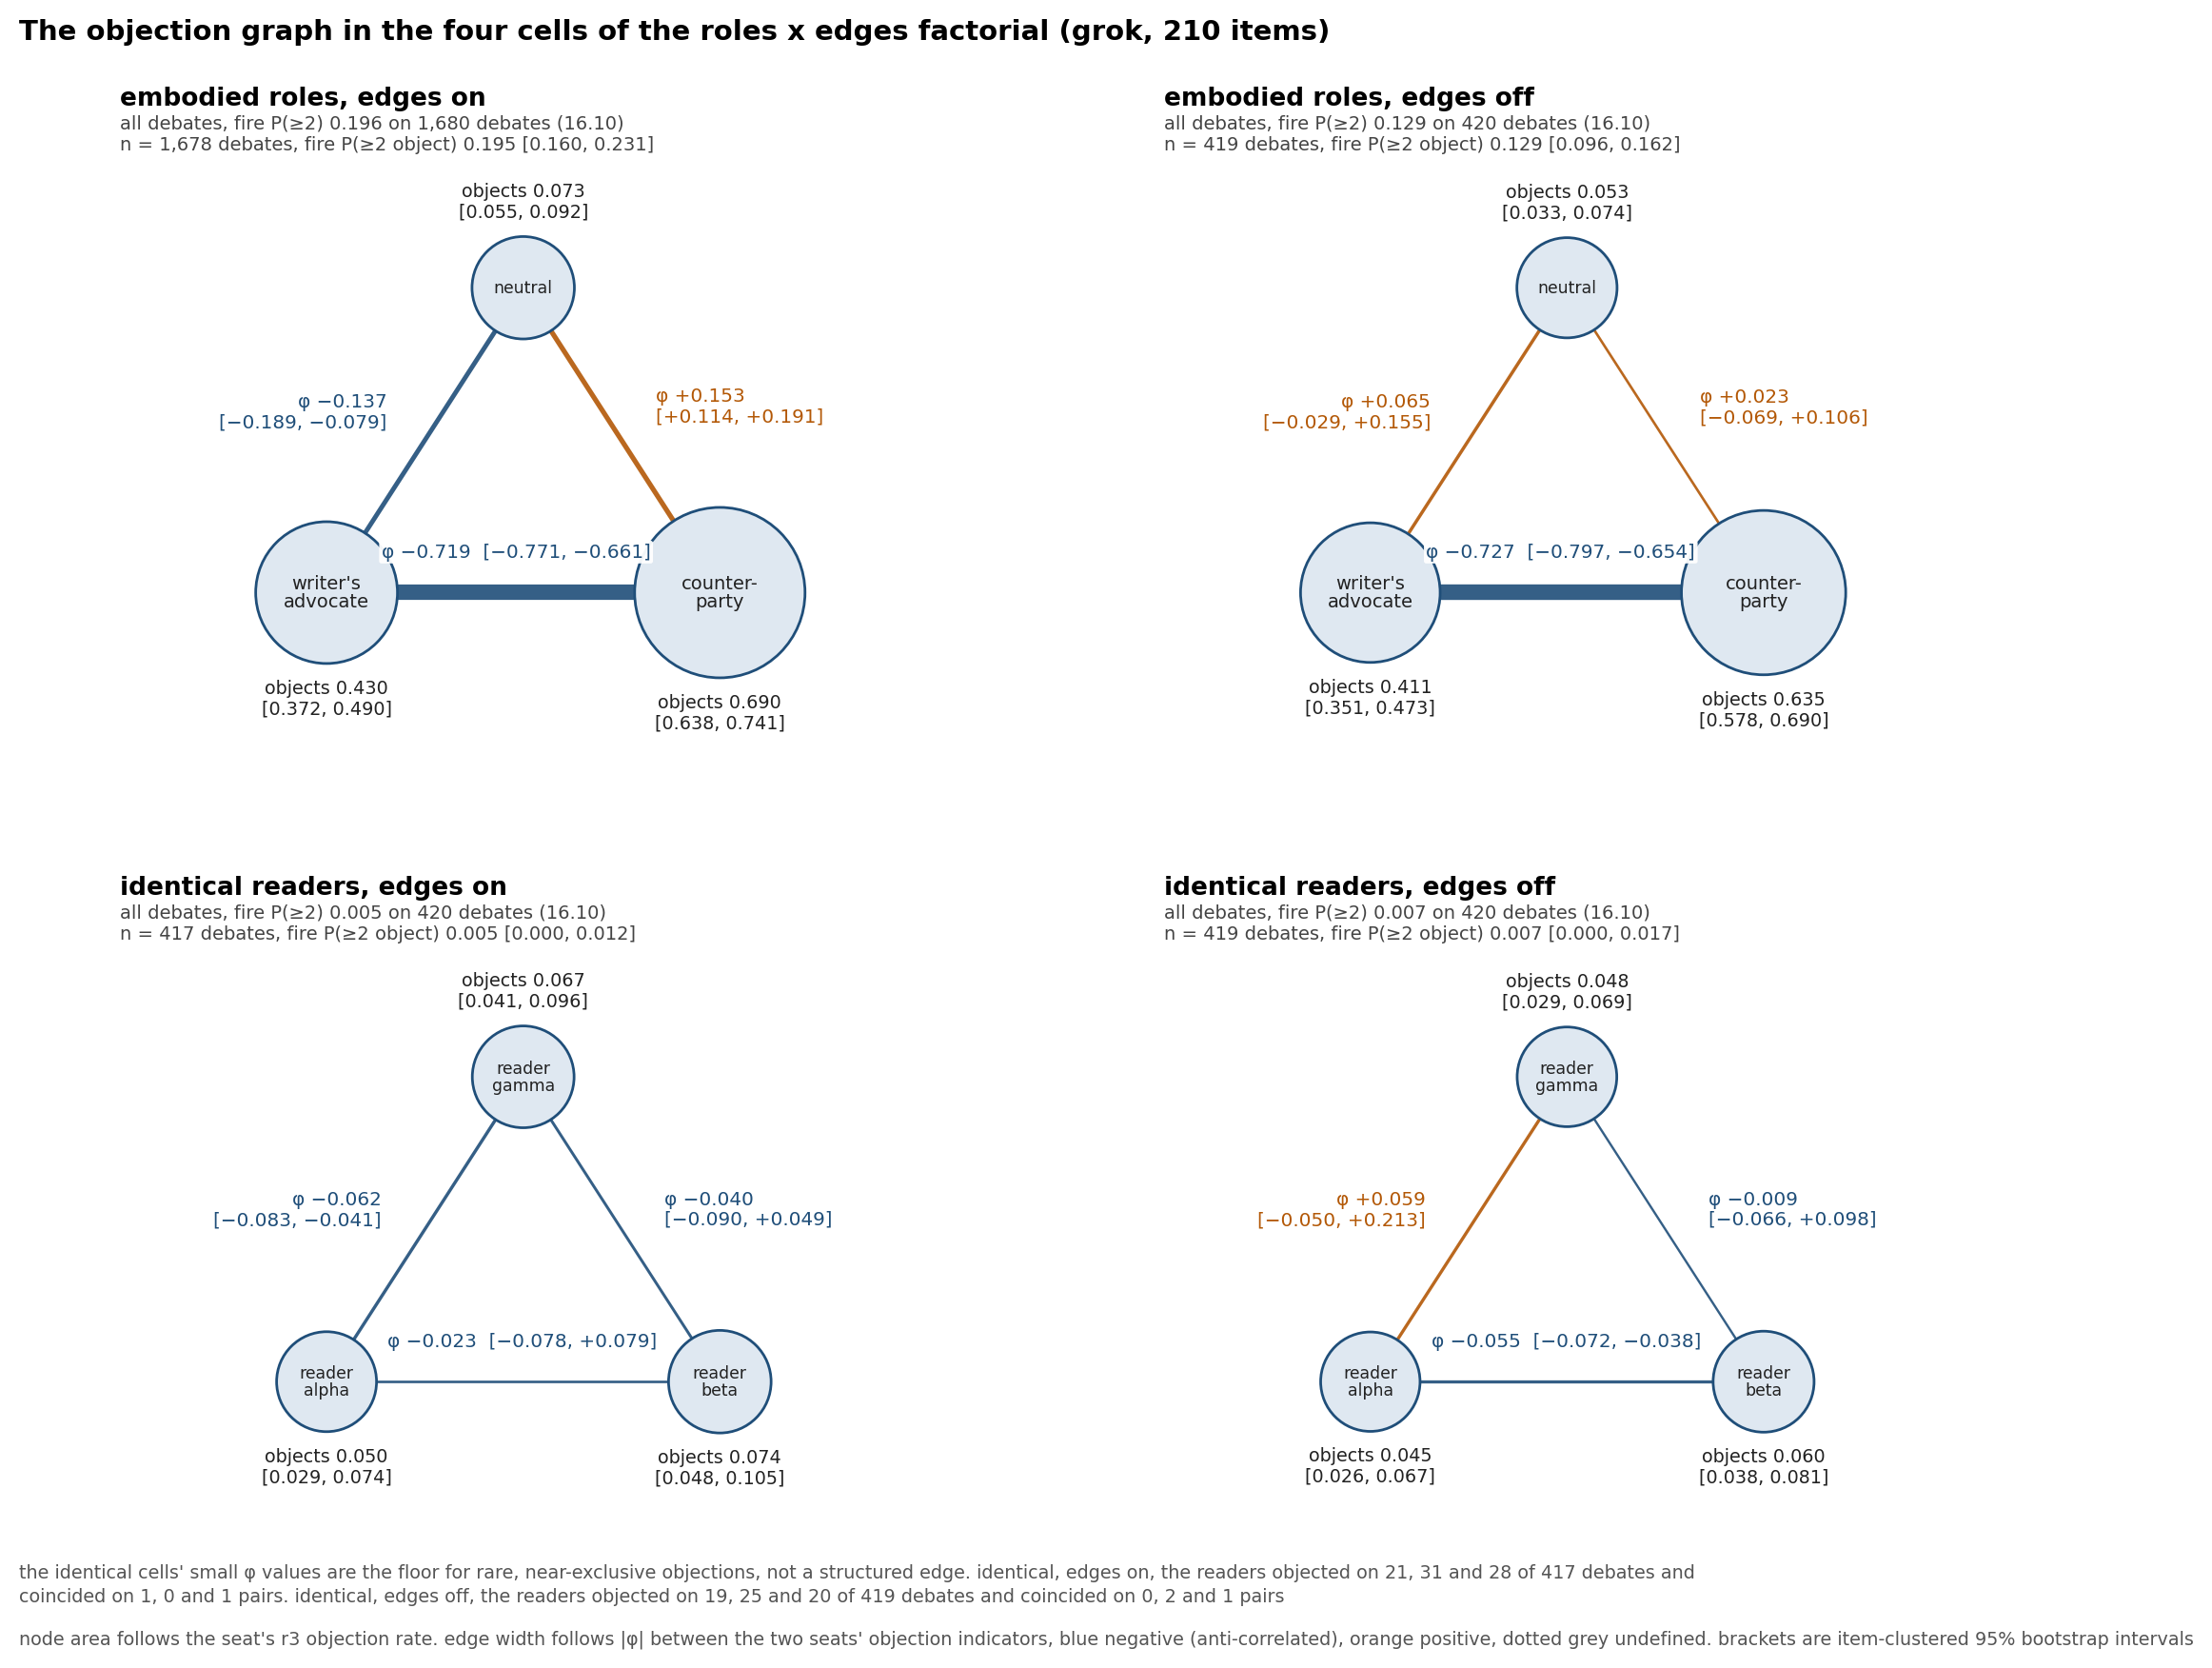
\includegraphics[width=\linewidth]{figures/g2_cells.png}
\caption{The objection graph in the four cells of the roles by edges
factorial on grok, 210 items. Node area follows each seat's r3 objection rate
and edge width follows the absolute $\phi$ between two seats' objection
indicators, blue negative and orange positive. The two embodied cells carry
the anti-correlated advocate edge, $\phi$ $-0.719$ $[-0.771, -0.661]$ with
the read arcs and $-0.727$ $[-0.797, -0.654]$ without, and the counter fires
on 0.196 and 0.129 of debates. The two identical-reader cells carry no edge
and the counter fires on 0.005 and 0.007. The structure follows the roles and
survives the removal of every exchange. The small negative $\phi$ values in
the identical cells are the floor for rare and near-exclusive objections, not
a structured edge, since the readers objected on 21, 31 and 28 of 417 debates
with the arcs and on 19, 25 and 20 of 419 without, and coincided on at most
two pairs.}
% make_graph_figures.py g2, emergent_graphs.json communities.{grok_aita,
% grok_aita_noedge, grok_aita_identical, grok_aita_identical_noedge}
% .populations.s2_codable.graphs.all (nodes.*.objection_rate, edges.*.phi,
% fire_rate) and .raw.fire_rate (equal to topology_2x2_analysis.json to 1e-9).
% 16.10 RESULTS, role-lock L4147, fire rates 0.196 / 0.129 / 0.005 / 0.007 L4149,
% n fired 329 / 54 / 2 / 3 L4151, structure survives edge removal L4175.
% identical-cell objection counts and coincidences from nodes.*.n_objected and
% edges.*.table.both (artefact only, not a prereg line).
\label{fig-g2-cells}
\end{figure}

\begin{figure}[t]
\centering
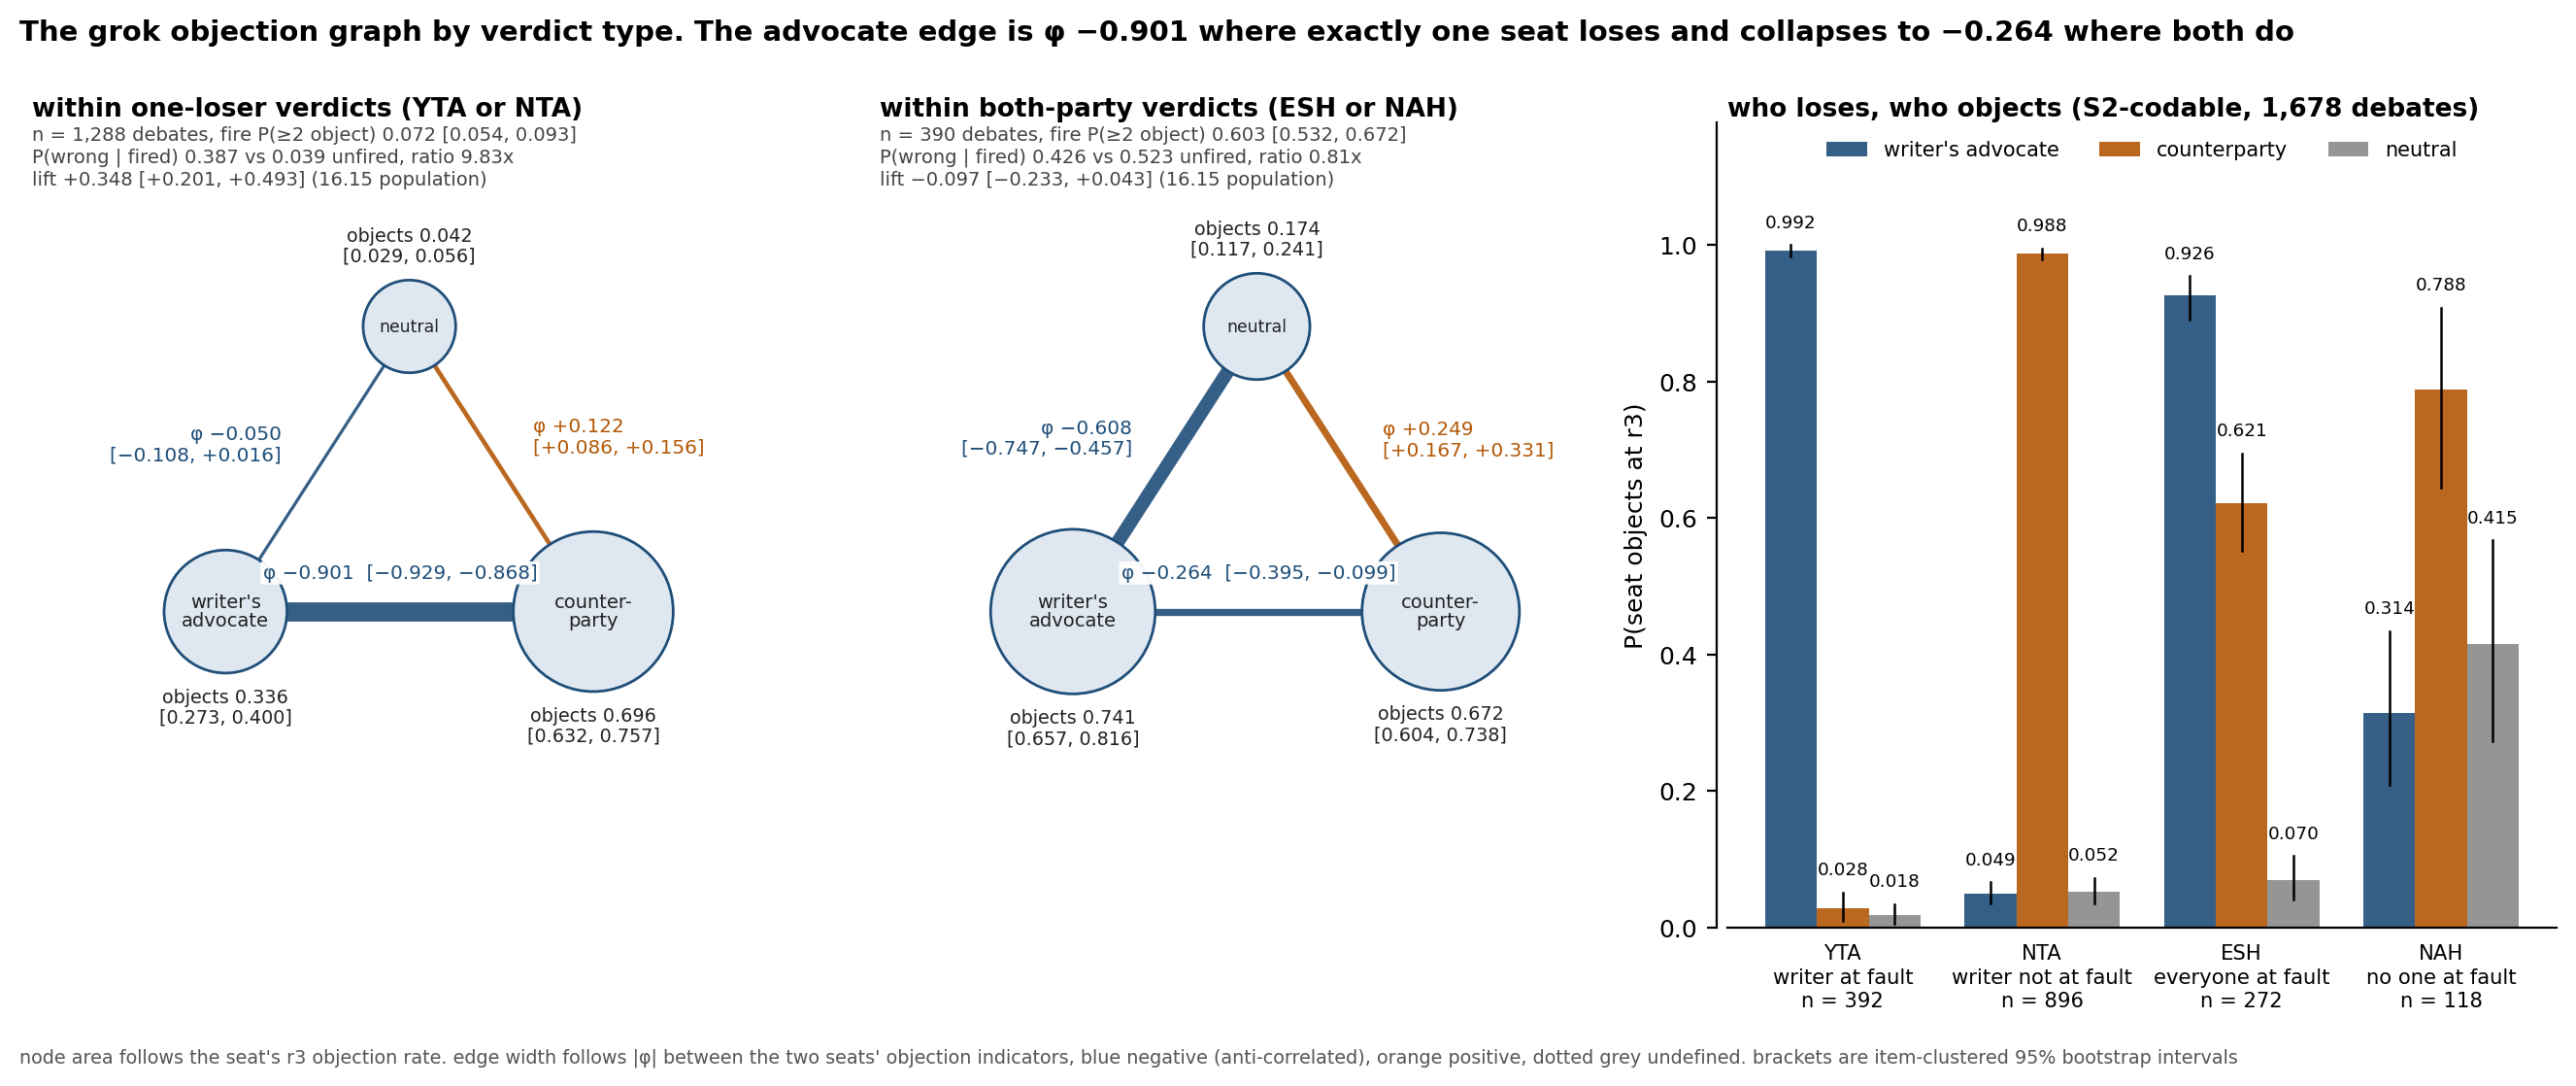
\includegraphics[width=\linewidth]{figures/g3_by_verdict.png}
\caption{The grok objection graph by verdict type. Within one-loser
verdicts, YTA or NTA, 1,288 debates, the advocate edge is $\phi$ $-0.901$
$[-0.929, -0.868]$, exactly one seat objects on 0.922 of debates, the counter
fires on 0.072 and a flagged debate is wrong 0.387 against 0.039 unflagged,
ratio 9.83, lift $+0.348$ $[+0.201, +0.493]$. Within both-party verdicts, ESH
or NAH, 390 debates, the edge collapses to $-0.264$ $[-0.395, -0.099]$, the
counter fires on 0.603 and the lift is $-0.097$ $[-0.233, +0.043]$. The bars
show who loses and who objects. The writer's advocate objects on 0.992 of YTA
and the counterparty on 0.988 of NTA, the with-interest objections that carry
nothing, while the counterparty objects on 0.028 of YTA and the writer's
advocate on 0.049 of NTA, the against-interest objections that carry the
case. On ESH both advocates object, and on NAH the counterparty objects on
0.788 while the writer's advocate still objects on 0.314, so both types
flood. The pooled anti-correlation is carried by which seat loses.}
% make_graph_figures.py g3, emergent_graphs.json communities.grok_aita
% .populations.s2_codable.graphs.{one_loser, both_party} and .who_loses.{YTA,
% NTA, ESH, NAH}.objection_rate.*, sensor strata from
% .populations.s1_s2_codable.sensor.strata.{one_loser, both_party}.
% 16.12 flooding table L3666 to L3668 (0.922 / 0.072 / -0.901, ESH 0.614, NAH
% 0.576), 16.15.1 strata L4275 to L4276 (0.387 vs 0.039, 9.83x, +0.348, and
% -0.097 within both-party), who loses L5003 to L5005 (0.992 of YTA, 0.988 of
% NTA). the both-party fire rate 0.603 is the s2_codable both_party block and
% agrees with flooding_analysis.json table_16_12.rows.both_party.p_two_plus.
\label{fig-g3-by-verdict}
\end{figure}

\begin{figure}[t]
\centering
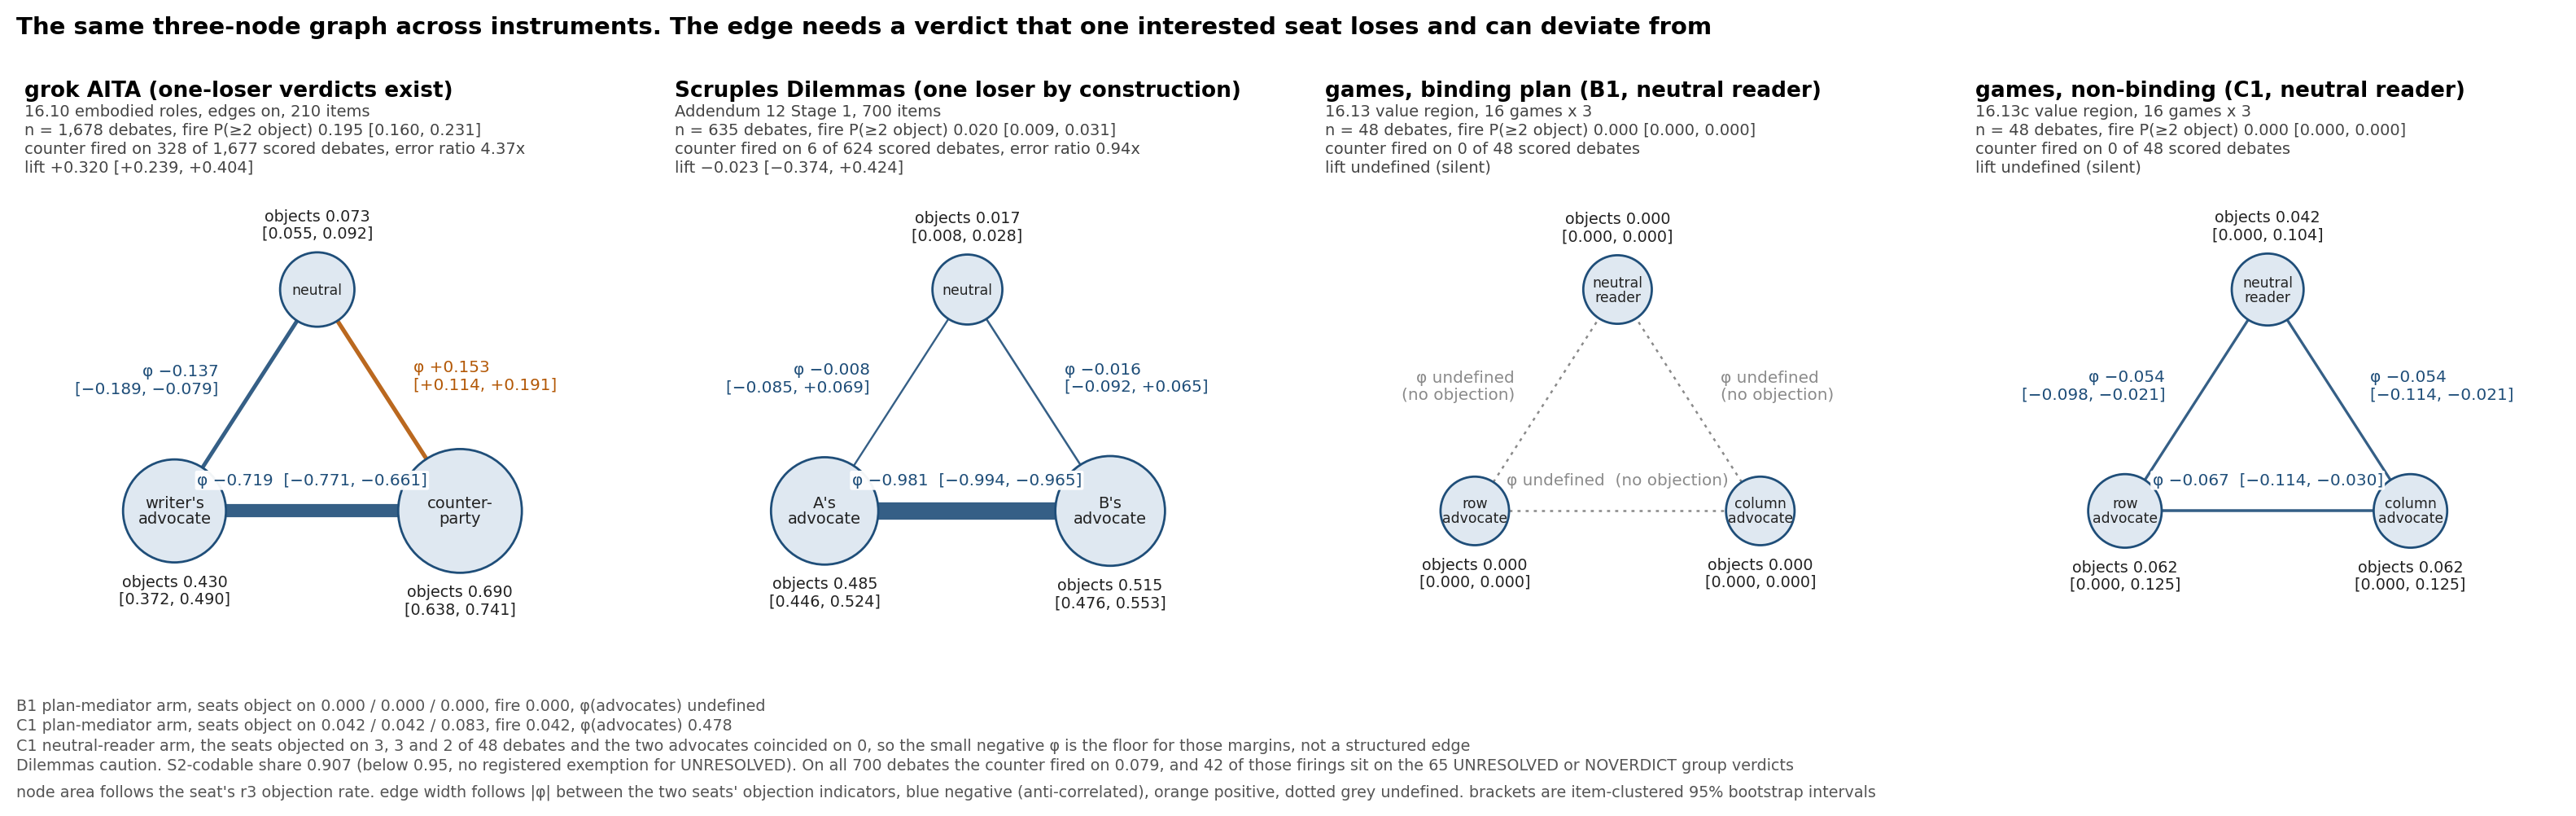
\includegraphics[width=\linewidth]{figures/g4_instruments.png}
\caption{The same three-node graph across instruments. On grok AITA
one-loser verdicts exist, the pooled advocate edge is $\phi$ $-0.719$
$[-0.771, -0.661]$, the counter fires on 0.195 of the 1,678 codable debates
and its pooled lift is $+0.320$ $[+0.239, +0.404]$. On the Scruples Dilemmas
exactly one advocate loses by construction and the edge is $-0.981$
$[-0.994, -0.965]$, yet the counter fires on 13 of 635 codable debates and on
6 of the 624 scored debates, on which the lift is $-0.023$ $[-0.374, +0.424]$.
That silence was not predicted (the record expected about 30 firings and got
6), and the account that the verdict space is binary so the favoured advocate
has no partial concession to move to is post hoc. That run is read with
caution because its S2-codable share is 0.907 and 42 of its 55 raw firings
sit on the 65 UNRESOLVED or NOVERDICT verdicts. Under a binding joint plan
(B1, 16 games by three samples) no seat objects on any of 48 debates and every
$\phi$ is undefined. Under the non-binding plan (C1) the seats object on 3, 3
and 2 of 48 debates and never coincide, so the small negative $\phi$ is the
floor for those margins. The edge needs a verdict that one interested seat
loses and can deviate from, and one loser is necessary but not sufficient.}
% make_graph_figures.py g4, emergent_graphs.json communities.{grok_aita,
% grok_dilemmas, grok_games_binding_neutral, grok_games_nonbinding_neutral}
% .populations.s2_codable.graphs.all and .populations.s1_s2_codable.sensor.strata.all.
% pooled lift +0.320 L4277. Dilemmas 6 of 624 L2594 (Addendum 12 Stage 1 G1
% fire rate 0.010), actuator null L2613, codable share 0.907 from
% communities.grok_dilemmas.guards.checks.s2_codable_share (status
% READ_WITH_CAUTION, no registered exemption for UNRESOLVED). B1 zero
% objections L4753, both arms 1.000 L4743 (game_B1_analysis.json). C1 objection
% counts 3 / 3 / 2 of 48 and zero coincidences from nodes.*.n_objected and
% edges."advocate_1|advocate_2".table.both (artefact only). planner-arm
% footnote values from the *_planner communities.
\label{fig-g4-instruments}
\end{figure}

\begin{figure}[t]
\centering
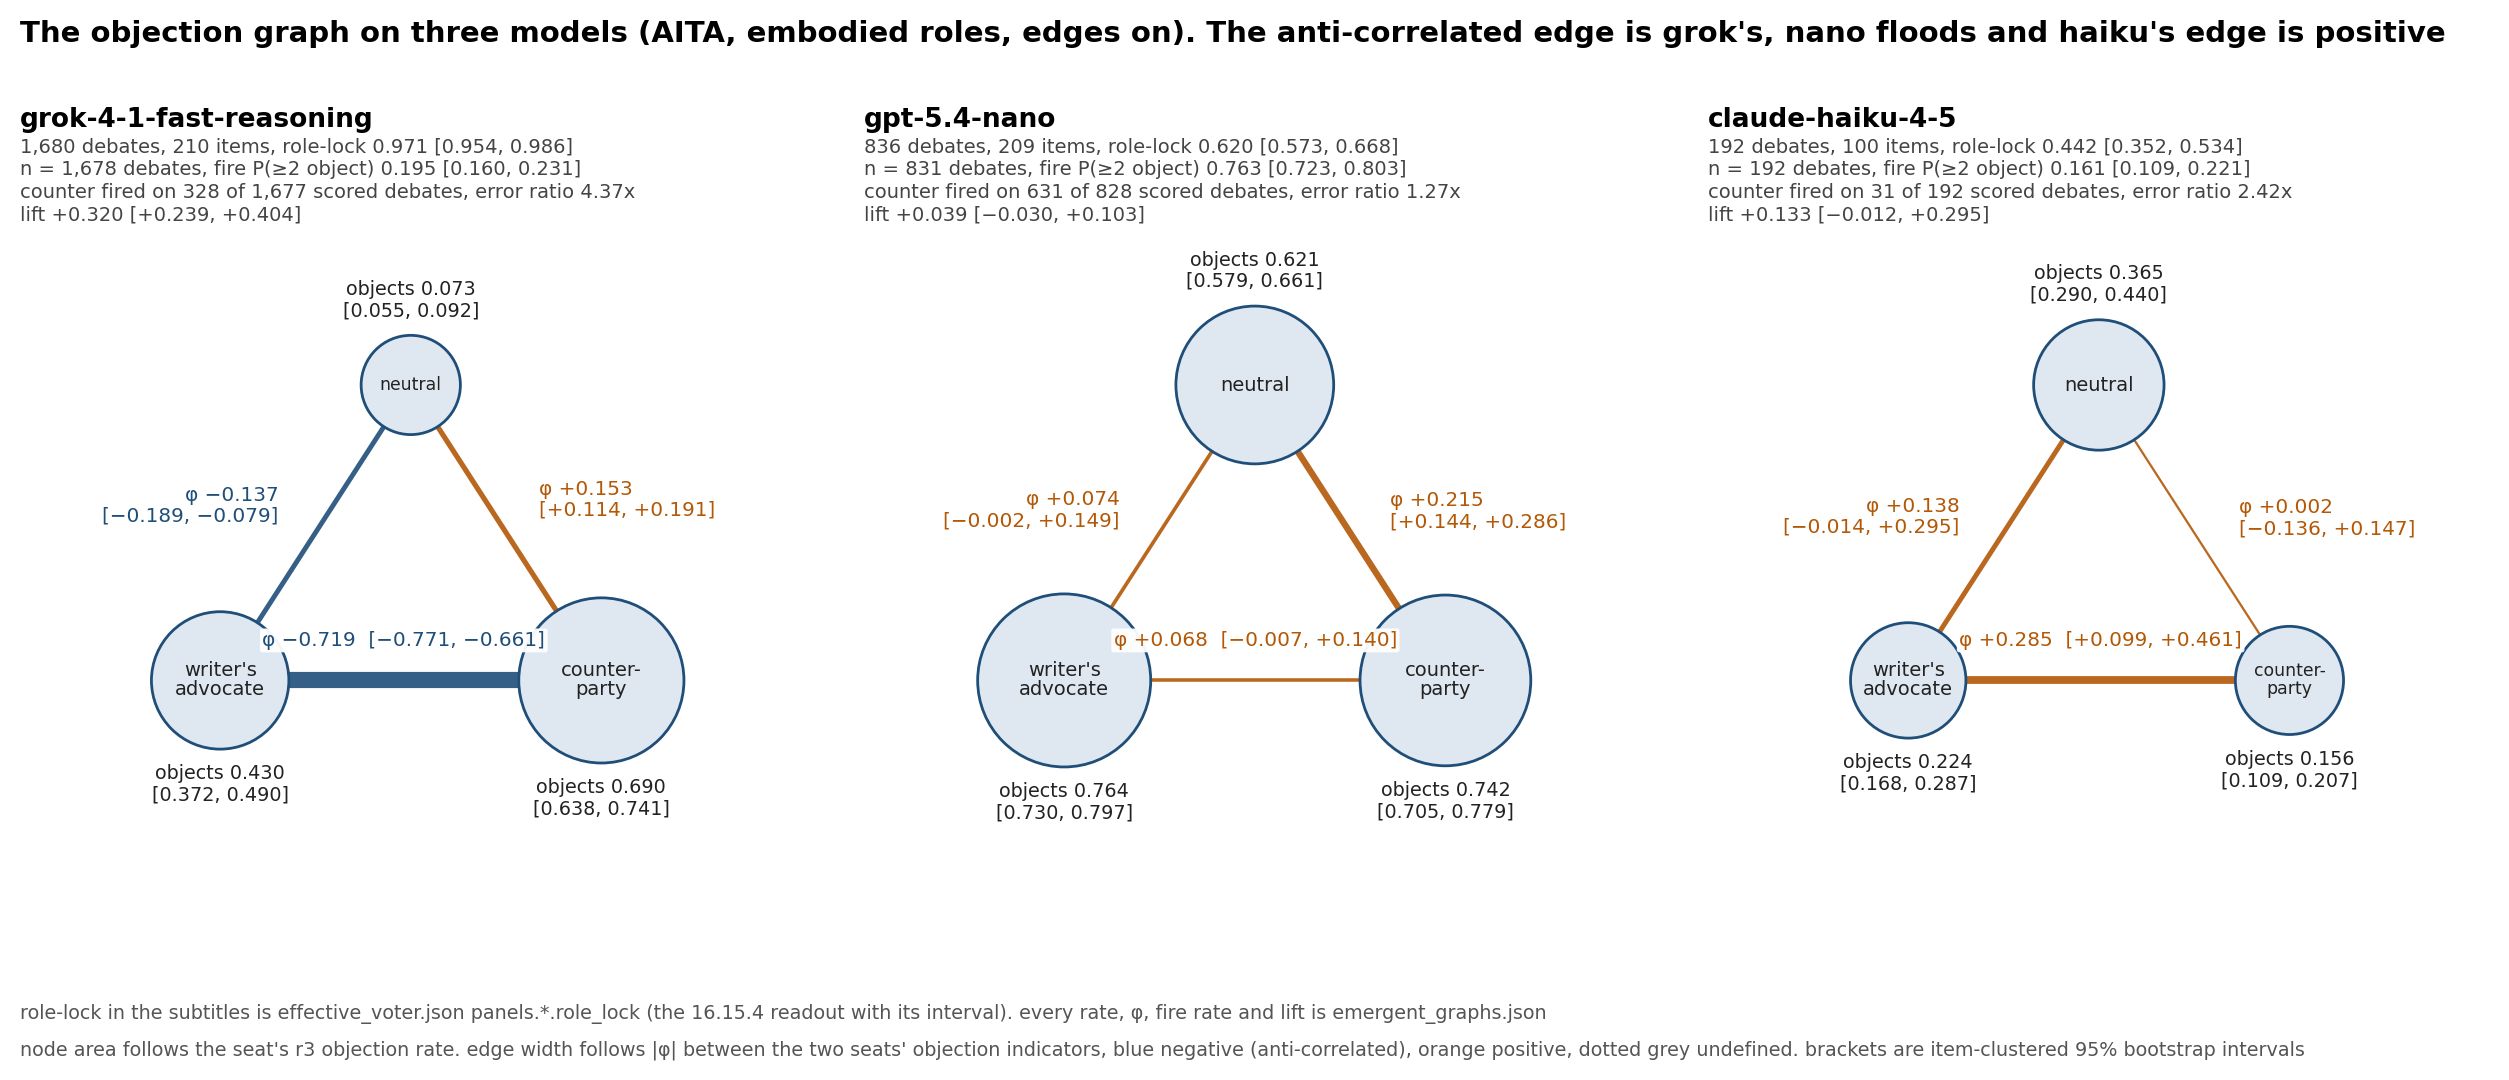
\includegraphics[width=\linewidth]{figures/g5_models.png}
\caption{The objection graph on three models, AITA with embodied roles and
the read arcs on. The anti-correlated edge is grok's, $\phi$ $-0.719$
$[-0.771, -0.661]$ at role-lock 0.971 $[0.954, 0.986]$. Nano floods, every
seat objecting on 0.62 to 0.76 of debates with the counter firing on 0.763 and
the advocate edge at $+0.068$ $[-0.007, +0.140]$, at role-lock 0.620
$[0.573, 0.668]$. Haiku's advocates object together, $\phi$ $+0.285$
$[+0.099, +0.461]$ at role-lock 0.442 $[0.352, 0.534]$, and its neutral seat
is the most frequent objector at 0.365. The edge is a property of the locked
model. Haiku is the best collective relative to its own seats and a weaker
sensor than grok, pooled lift $+0.133$ $[-0.012, +0.295]$ against $+0.320$
$[+0.239, +0.404]$, and nano, whose advocates flood, is the weakest at
$+0.039$ $[-0.030, +0.103]$.}
% make_graph_figures.py g5, emergent_graphs.json communities.{grok_aita,
% nano_aita, haiku_aita}.populations.s2_codable.graphs.all and
% .populations.s1_s2_codable.sensor.strata.all. role-lock and its interval from
% effective_voter.json panels.{grok, nano, haiku}.role_lock (16.15.4 table,
% grok L4496, nano L4498, haiku L4499), n_debates cross-checked
% between the two artefacts under --check. nano fire 0.763 and haiku phi
% +0.285 are artefact values with no prereg line (emergent_graphs.json only).
% pooled sensor lifts from communities.{grok_aita, haiku_aita, nano_aita}
% .populations.s1_s2_codable.sensor.strata.all.lift (grok L4277).
\label{fig-g5-models}
\end{figure}

\begin{figure}[t]
\centering
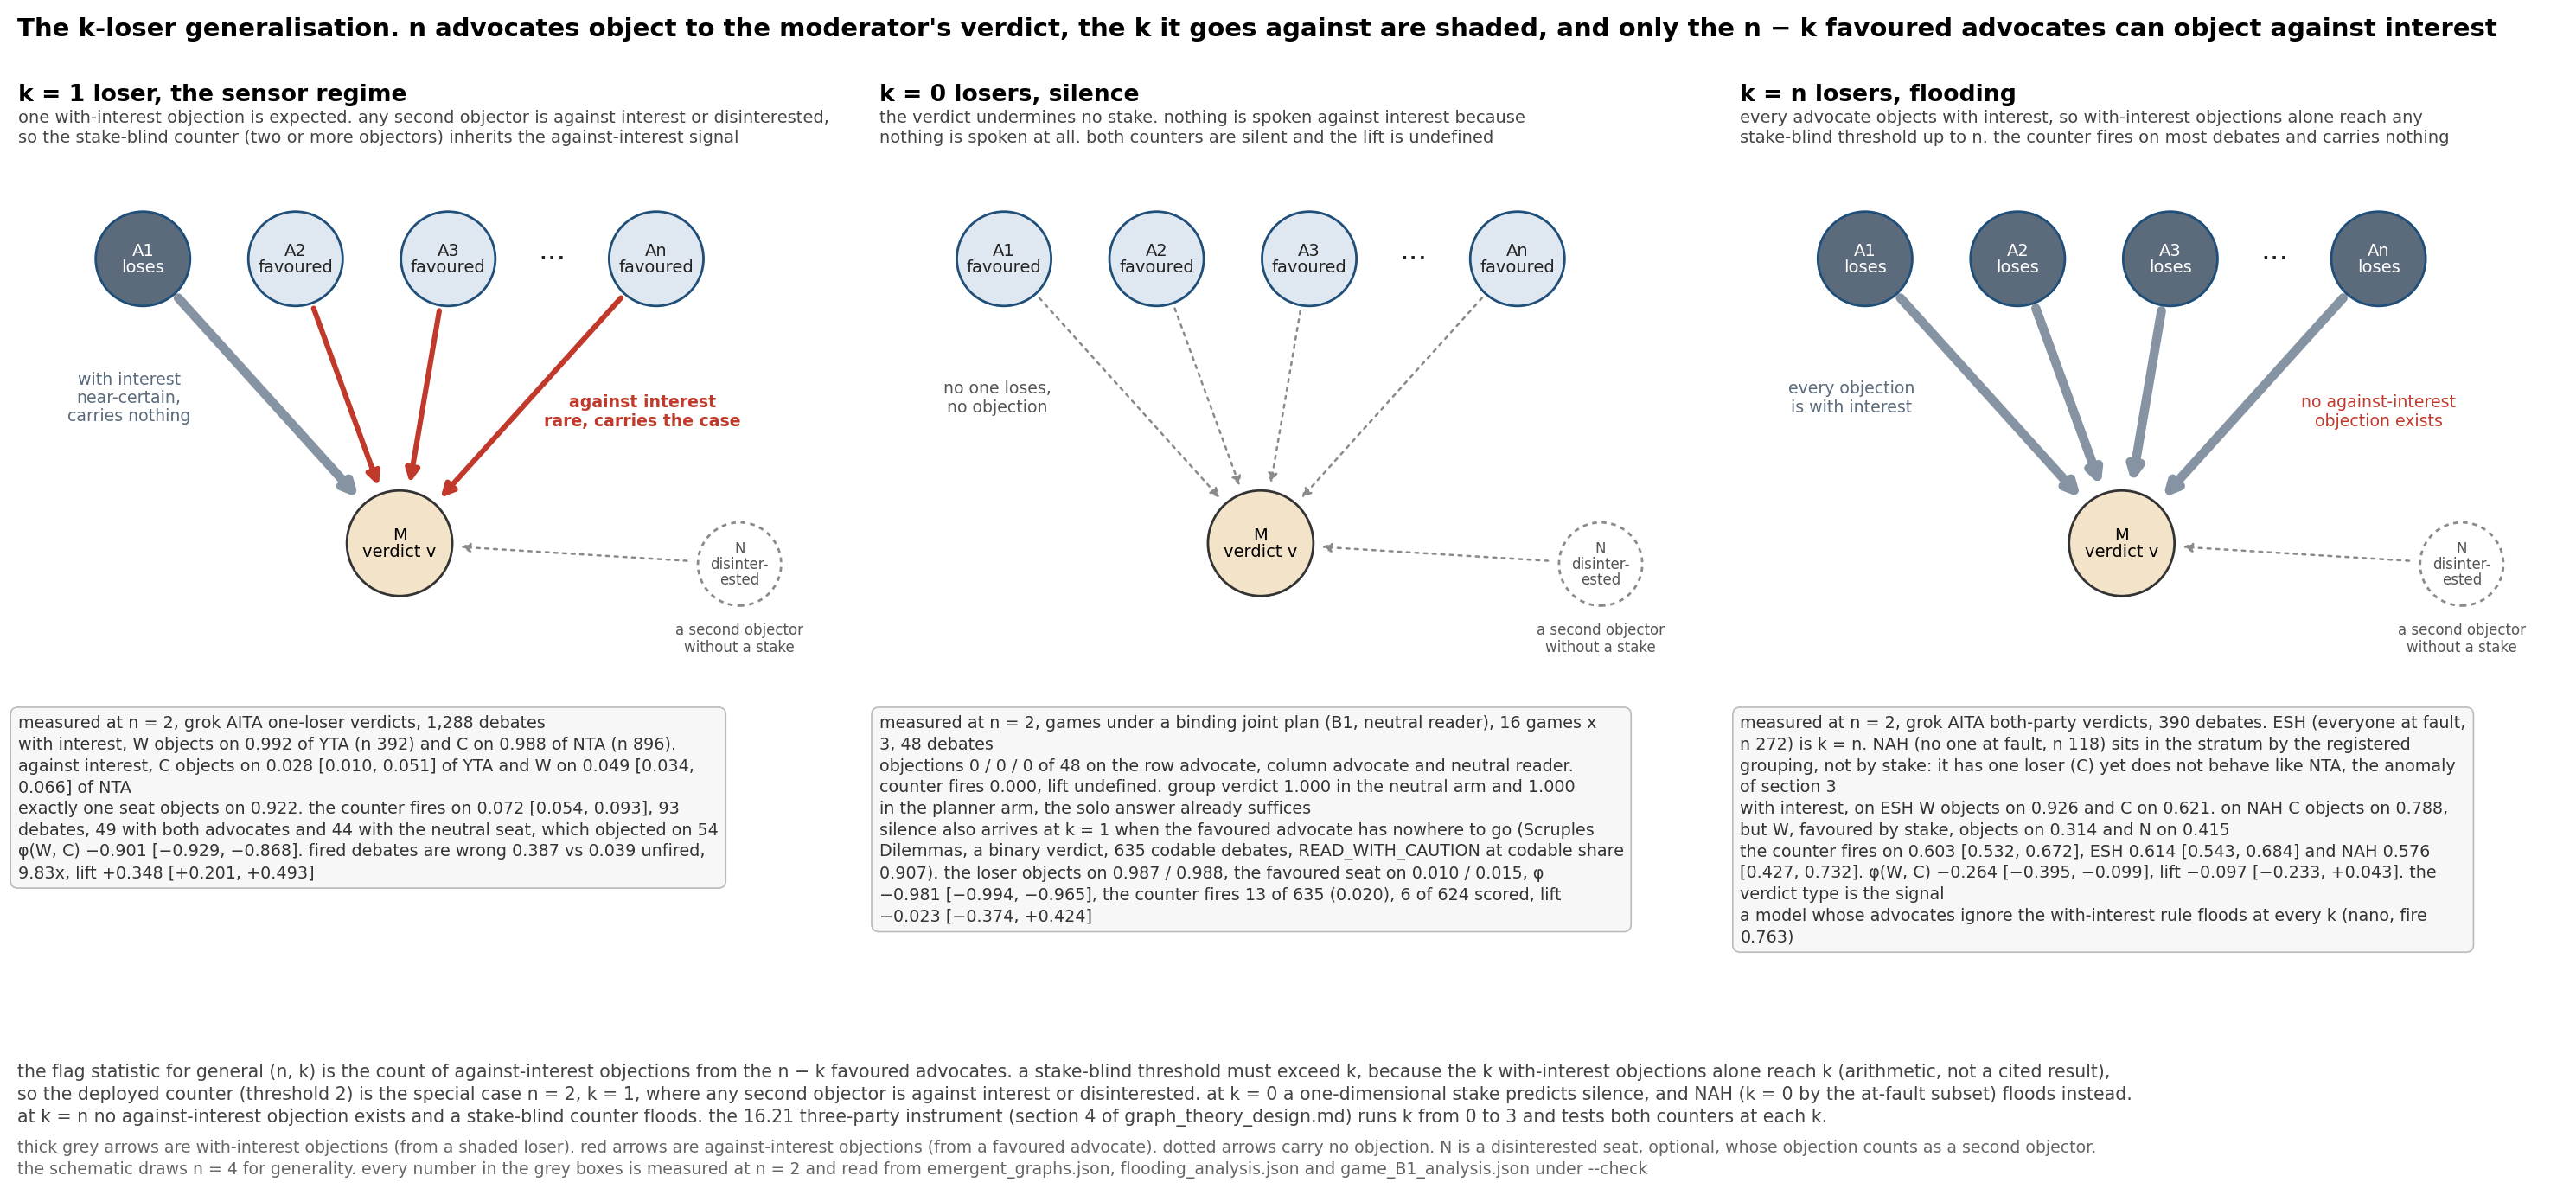
\includegraphics[width=\linewidth]{figures/g5_n_perspectives.png}
\caption{The $k$-loser generalisation. $n$ advocates object to the
moderator's verdict $v$, the $k$ advocates the verdict goes against are
shaded, their with-interest objections are the thick grey arrows, and the
against-interest objections from the $n-k$ favoured advocates are the red
arrows. The flag statistic for general $(n, k)$ is the count of
against-interest objections, and a stake-blind threshold must exceed $k$
because the $k$ with-interest objections alone reach it, a counting argument
of this design, and \citet{feddersen1998convicting} are cited only for the half
they support, that a unanimity trigger is the wrong rule under strategic
voters. The deployed counter is the special case
$n = 2$, $k = 1$, where any second objector is against interest or
disinterested. At $k = 1$ on grok AITA the with-interest objection is
near-certain (0.992 of YTA, 0.988 of NTA), the against-interest objection is
rare (0.028 and 0.049), exactly one seat objects on 0.922 of the 1,288
one-loser debates, the counter fires on 0.072 and lifts error detection by
$+0.348$ $[+0.201, +0.493]$, 9.83 times. At $k = 0$ under a binding joint plan
no seat objects on any of 48 debates and both arms score 1.000, and silence
also arrives at $k = 1$ on the Scruples Dilemmas, which fire on 13 of 635
codable debates and 6 of the 624 scored debates, lift $-0.023$
$[-0.374, +0.424]$, a silence the record did not predict and for which the
"nowhere to go" account is post hoc. At $k = n$ on both-party verdicts every
objection is with interest, the counter fires on 0.603 (ESH 0.614, NAH 0.576)
and its lift is $-0.097$ $[-0.233, +0.043]$. NAH sits in that stratum by the
registered grouping and not by stake, since under the stake definition it has
one loser and under the at-fault subset it is $k = 0$, and it floods rather
than falling silent, with the writer's advocate objecting on 0.314 of it. So
the $k = 0$ prediction for 16.21 is conditional, silence if the stake is
one-dimensional and flooding at the NAH level if it is not. A model whose
advocates ignore the with-interest rule floods at every $k$ (nano, 0.763). The
schematic draws $n = 4$ and every number is measured at $n = 2$. The 16.21
three-party instrument runs $k$ from 0 to 3.}
% make_graph_figures.py g5n. k = 1 values from emergent_graphs.json
% communities.grok_aita.populations.s2_codable.graphs.one_loser (n, p_exactly_one,
% fire_rate, edges table.both = 49 of 93 firings, nodes.third.n_objected = 54)
% and .who_loses.{YTA, NTA}.objection_rate.* (L5003 to L5005, L3666), sensor
% strata.one_loser L4275. k = 0 from communities.grok_games_binding_neutral
% (L4753) and game_B1_analysis.json arms.*.accuracy.group.final.all (L4743).
% Dilemmas from communities.grok_dilemmas (L2594, codable share 0.907). k = n
% from graphs.both_party, who_loses.{ESH, NAH} and flooding_analysis.json
% table_16_12.rows.{ESH, NAH}.p_two_plus (L3667 to L3668), lift L4276. nano
% fire 0.763 from communities.nano_aita (artefact only). the threshold rule is
% the design's own counting argument; Feddersen and Pesendorfer 1998 supports
% only the "not unanimity" half (advocacy_refs.bib, references.bib).
\label{fig-g5-n-perspectives}
\end{figure}

\begin{figure}[p]
\centering
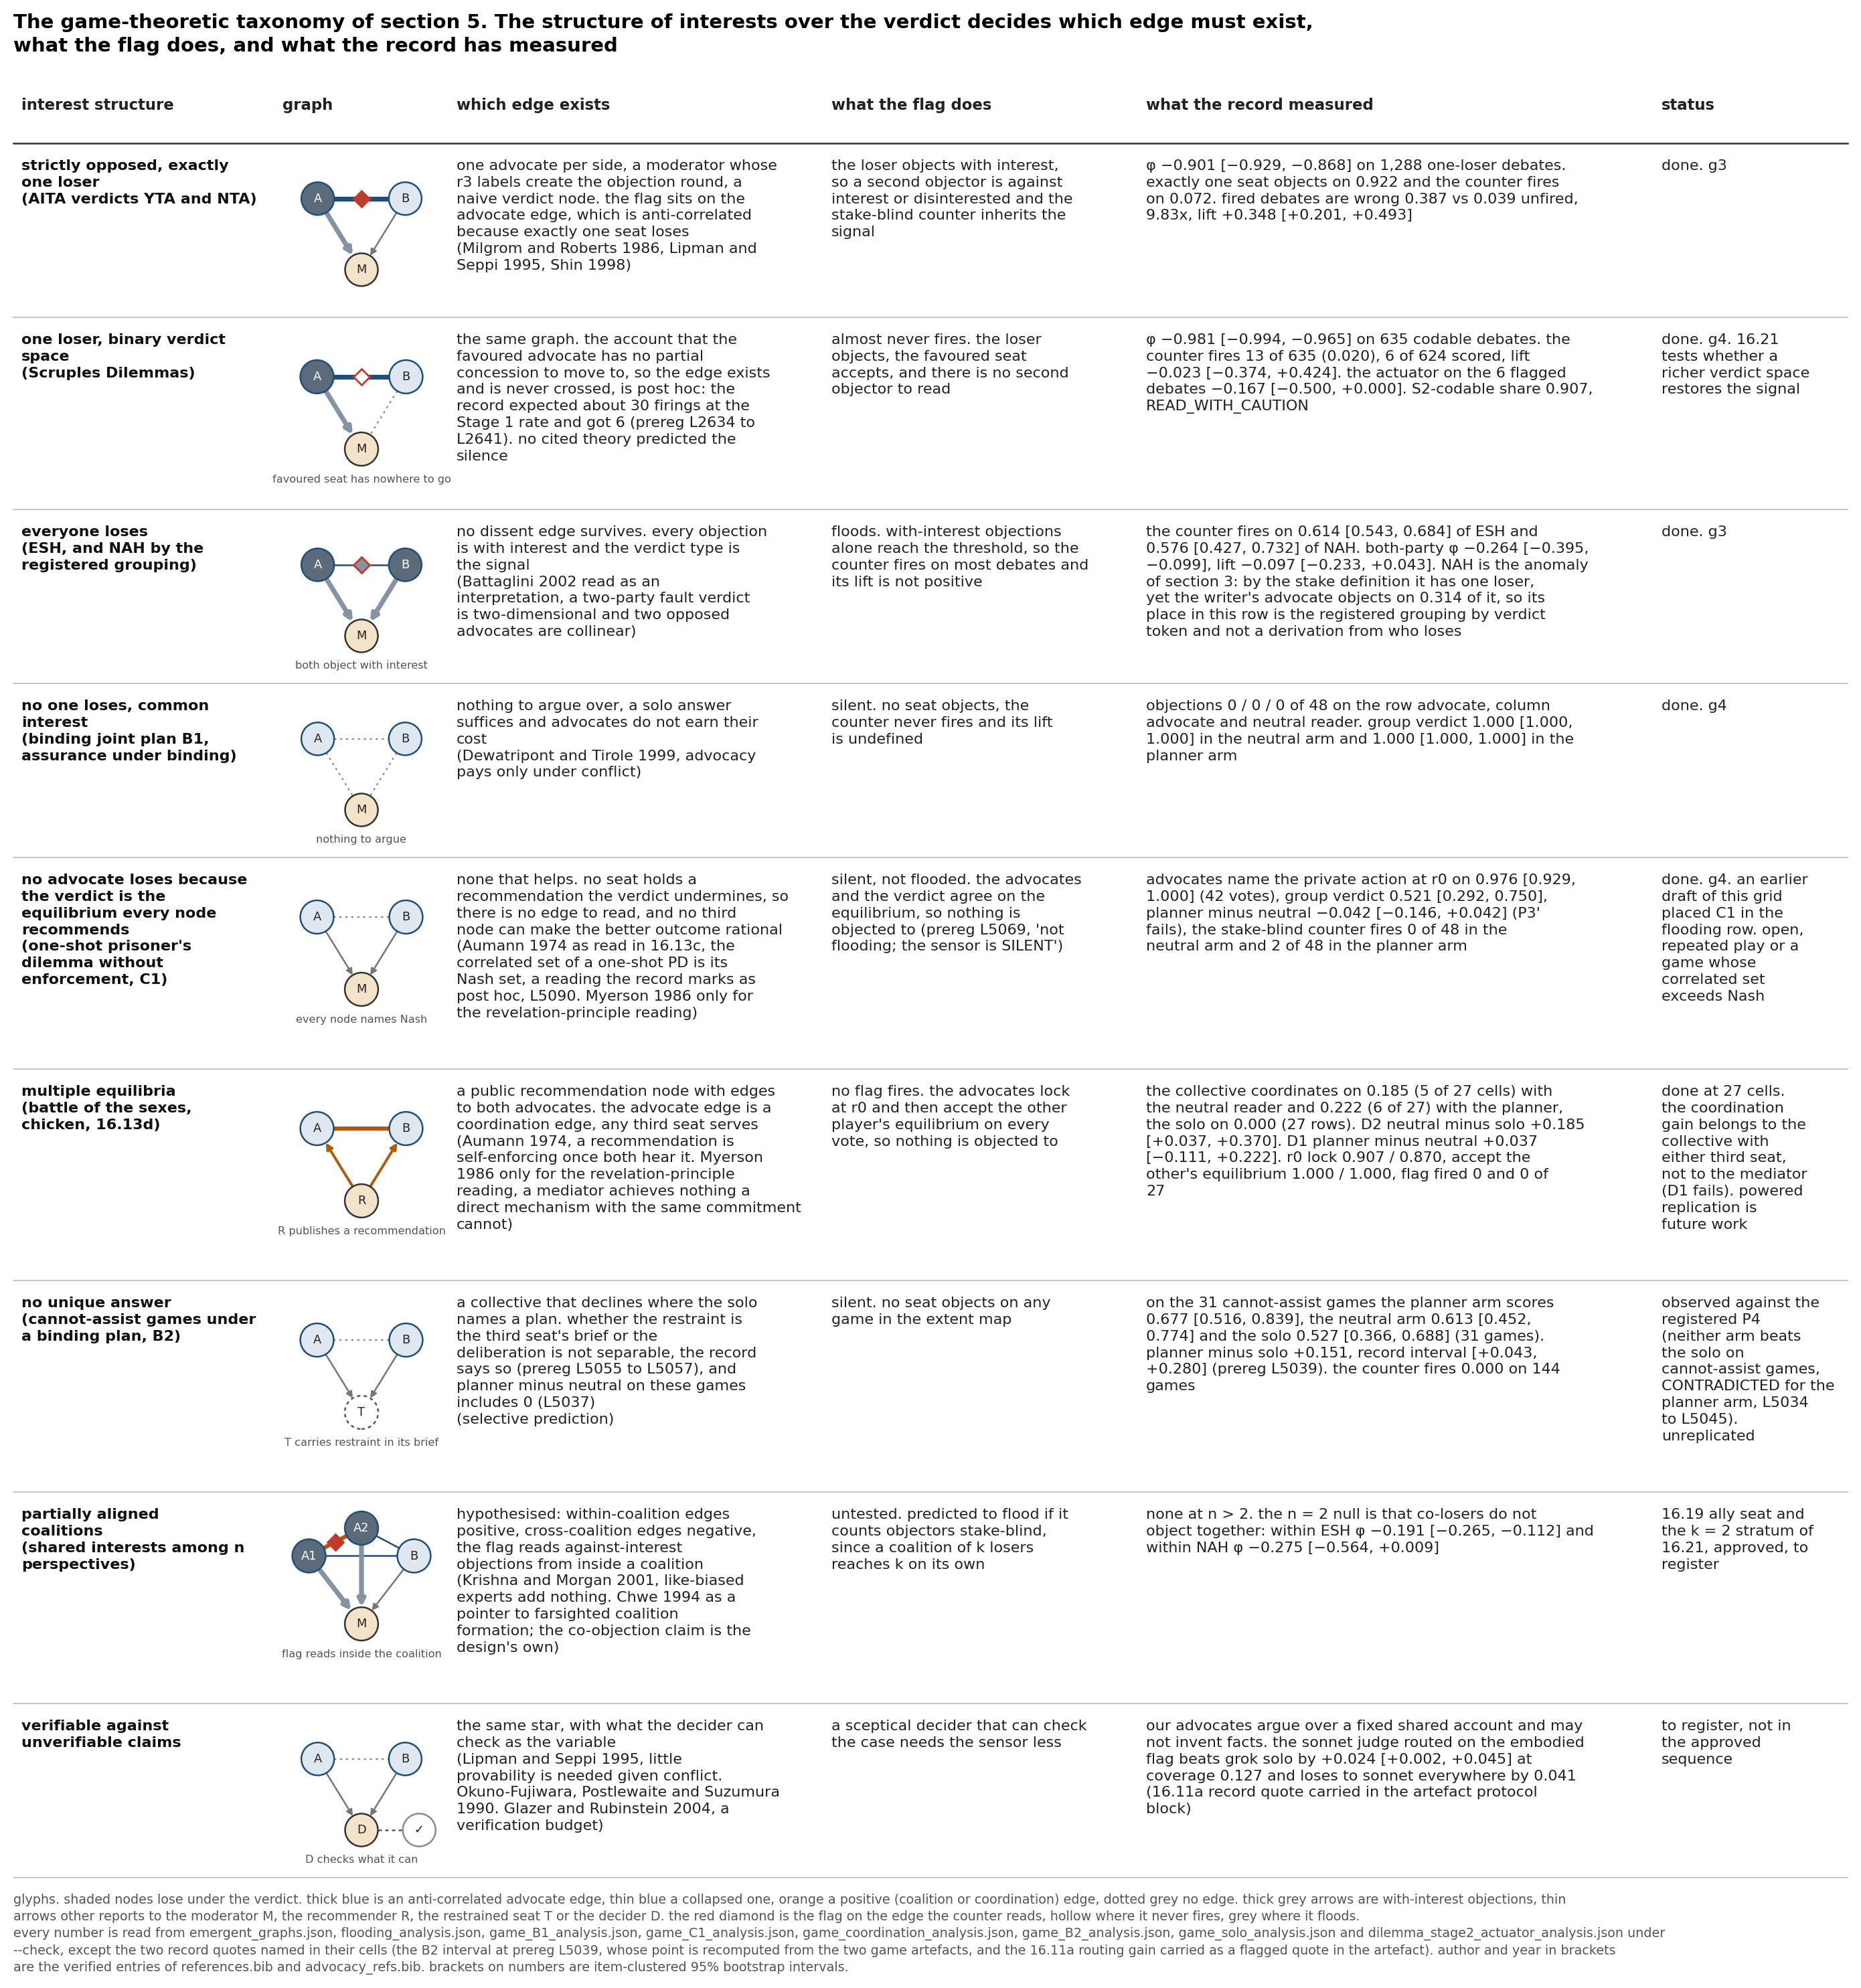
\includegraphics[width=\linewidth]{figures/g6_taxonomy.png}
\caption{The game-theoretic taxonomy. One row per structure of interests over
the verdict, with the requisite graph as a glyph, which edge must exist, what
the flag does and what the record measured. Where exactly one advocate loses
the dissent edge is anti-correlated and the flag reads it
\citep{milgrom1986relying, lipman1995robust, shin1998adversarial}, $\phi$
$-0.901$ and lift $+0.348$ on AITA. On the Dilemmas the edge exists and is
almost never crossed, $\phi$ $-0.981$ and 13 firings in 635 codable debates (6
of 624 scored), a silence no cited theory predicted, for which the account
that the loser's opponent has no partial concession is post hoc. Where everyone loses
the edge collapses and the flag floods, the counter firing on 0.614 of ESH
and 0.576 of NAH, and NAH sits in that row by the registered grouping rather
than by the stake definition, under which it has one loser and the writer's
advocate still objects on 0.314 of it. Where no one loses nothing is argued
and advocates do not earn their cost \citep{dewatripont1999advocates}, zero
objections on 48 debates. Where the verdict is the equilibrium every node
recommends, as in the one-shot prisoner's dilemma without enforcement, no
advocate loses and the sensor is silent rather than flooded, the counter
firing 0 of 48 in the neutral arm and 2 of 48 in the planner arm, since the
correlated set of that game is its Nash set, a reading of
\citet{aumann1974subjectivity} the record marks as one that should have been
made at registration, and no third node can make the better outcome rational
(\citealt{myerson1986multistage} is cited only for the revelation-principle
reading that a mediator achieves nothing a direct mechanism with the same
commitment cannot). Where the game has several equilibria a public
recommendation coordinates, the collective coordinating on 5 and 6 of 27 cells
against 0 for the solo with either third seat, while the mediator adds nothing
over a naive reader. Where no unique answer exists the collective declines to
name one more often than the solo, $+0.151$ on 31 cannot-assist games, an
outcome observed against the registered prediction that neither arm beats the
solo and not yet replicated, and whether the restraint belongs to the third
seat's brief or to the deliberation is not separable in the record. Coalitions
among $n$ perspectives are unmeasured at $n > 2$, with the $n = 2$ null that
co-losers do not object together (within ESH $\phi$ $-0.191$, within NAH
$-0.275$ $[-0.564, +0.009]$). \citet{krishna2001model} say like-biased experts
add nothing, and \citet{chwe1994farsighted} is a pointer to farsighted
coalition formation, the co-objection hypothesis being the design's own. The
verifiability of claims \citep{okunofujiwara1990strategic, glazer2004optimal}
is unmeasured. Two numbers are record quotes, the B2 interval and the 16.11a
routing gain.}
% make_graph_figures.py g6. row 1 emergent_graphs.json graphs.one_loser and
% sensor strata.one_loser (L3666, L4275). row 2 communities.grok_dilemmas and
% dilemma_stage2_actuator_analysis.json flagged.{n, delta, lo, hi} (L2594, L2613).
% row 3 flooding_analysis.json table_16_12.rows.{ESH, NAH}.p_two_plus (L3667 to
% L3668), graphs.both_party, sensor strata.both_party (L4276), who_loses.NAH.
% row 8 (coalitions) within-type phi from flooding_analysis.json
% table_16_12.rows.{ESH, NAH}.phi (L3667 to L3668, L5005 to L5006).
% row 4 communities.grok_games_binding_neutral nodes.*.n_objected (L4753) and
% game_B1_analysis.json arms.*.accuracy.group.final.all (L4743). row 5 (added
% 2026-09-13, C1 moved out of row 3, prereg L5069 "not flooding; the sensor is
% SILENT") game_C1_analysis.json readings.P1_prime.cgnb_game_neutral (private
% action 0.976, L5066), contrast.P3_prime (-0.042 [-0.146, +0.042], L5068),
% arms[0].accuracy.group.final.all, stake-blind counter 0 of 48 in the neutral
% arm (communities.grok_games_nonbinding_neutral) and 2 of 48 in the planner
% arm (communities.grok_games_nonbinding_planner). row 6
% game_coordination_analysis.json arms.{neutral, planner}.COORD (5 and 6 of 27
% recomputed as round(point x n_cells)), solo.COORD, contrasts "D2 neutral - solo,
% COORD" (+0.185 [+0.037, +0.370], L5159) and "D1 planner - neutral, COORD" (+0.037
% [-0.111, +0.222], L5158), LOCK_r0_prefers_own_equilibrium, ACCEPT_favours_other,
% FLAG_n_fired. row 7 game_B2_analysis.json arms.{0,1}.accuracy.group.final
% .by_region.cannot_assist (neutral 0.613, planner 0.677) and game_solo_analysis.json
% by_region.cannot_assist.accuracy (0.527); the point +0.151 is recomputed from these
% two and the interval [+0.043, +0.280] is the record quote at L5039, checked
% against the prereg text under --check. row 9 protocol.annotations
% .routing_gain_over_solo_16_11a, the flagged 16.11a record quote (L3621, L3623).
% author-year attributions on the figure are the verified entries of
% references.bib and advocacy_refs.bib.
\label{fig-g6-taxonomy}
\end{figure}

\begin{figure}[t]
\centering
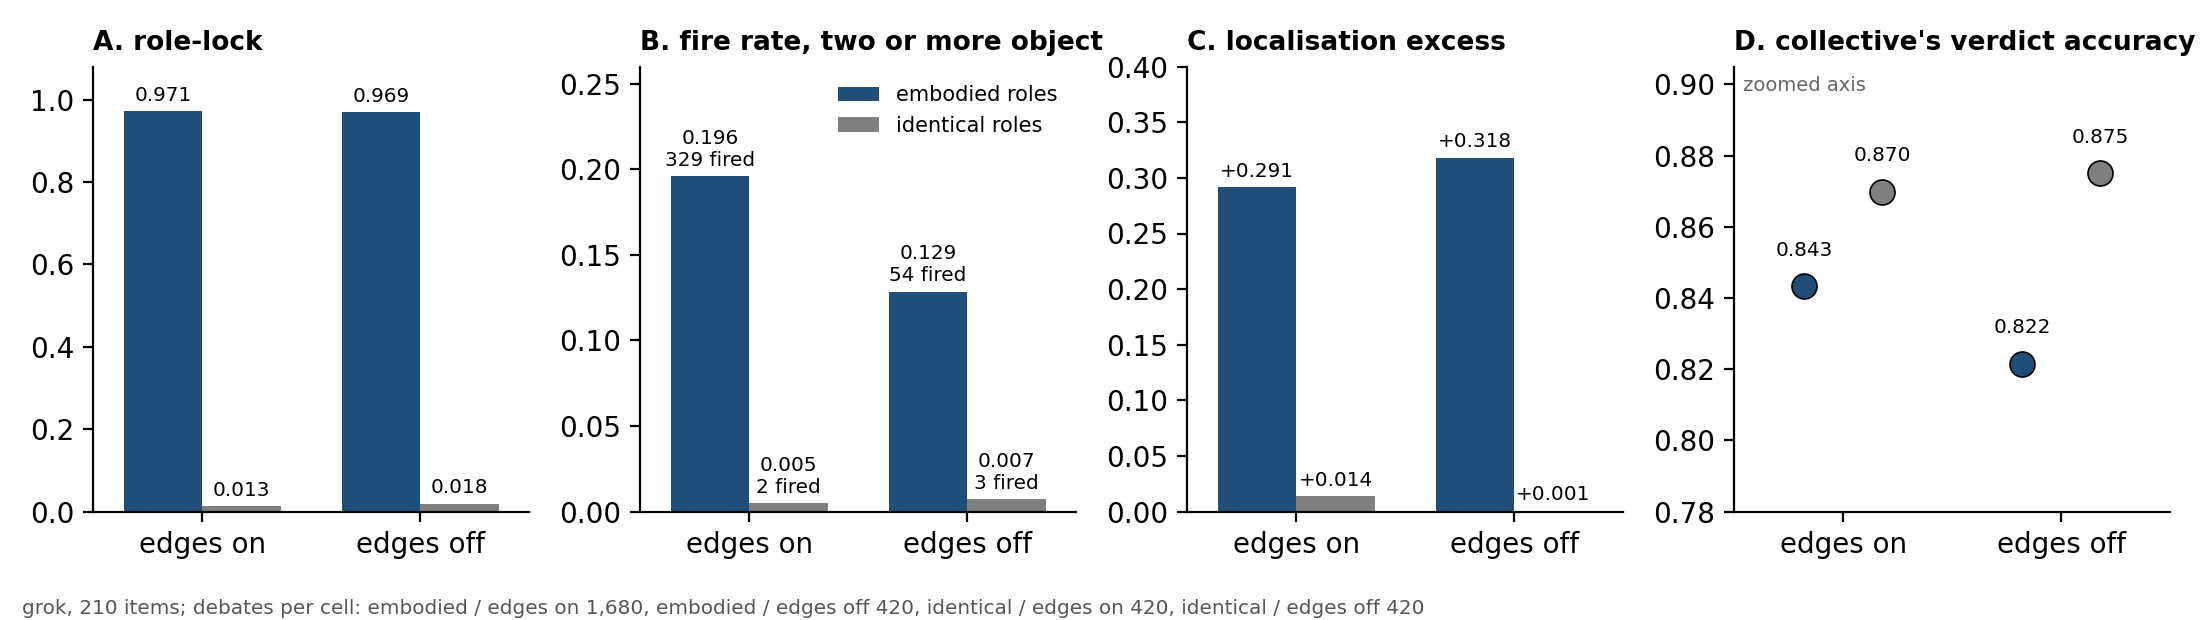
\includegraphics[width=\linewidth]{figures/fig6.png}
\caption{The roles by edges two-by-two on grok, the readouts behind
Figure~\ref{fig-g2-cells}. Role-lock, the fire rate of the counter, the
localisation excess and the collective's verdict accuracy per cell. Lock is
0.971 and 0.969 in the embodied cells and 0.013 and 0.018 in the identical
cells, the counter fires on 0.196 and 0.129 against 0.005 and 0.007, the
localisation excess is $+0.291$ and $+0.318$ against $+0.014$ and $+0.001$,
and the collective's verdict scores 0.843 and 0.822 against 0.870 and 0.875.
The structure follows the roles and survives the removal of every exchange,
and the identical-reader cells produce none of it and are the most accurate.}
% make_figures.py fig6, topology_2x2_analysis.json cells.*.role_lock,
% objection.fire_rate, objection.localisation_excess, aggregation.group_verdict_s2,
% n_debates and lift.n_fired (the item-matched cells block of Table tab-topology).
% 16.10 RESULTS L4147 to L4151 (lock, fire, n fired). the paired contrasts at
% L4192 to L4196 (identical/off minus embodied/on +0.030 [+0.012, +0.048],
% edges-off cost to the embodied S2 -0.023 [-0.042, -0.004]) are item-matched on
% 209 items and their per-cell S2 values (0.842, 0.872) differ from the cells
% block drawn here (0.843, 0.875) by 0.001 to 0.003. verified by
% `make_figures.py --check` (65 cross-artefact equalities, run 2026-09-13).
\label{fig-topology-readouts}
\end{figure}
